\appendix
\chapter{Anexo}

\section{Hibridación sp2}
\label{sec:hibridacion_sp2}

En la hibridación sp2, los orbitales 2s, 2px y 2py del carbono, se combinan para formar 3 orbitales sp2 dispuestos en un plano con un ángulo de 120° entre ellos (ver figura \ref{fig:sp2_hybrid}), dejando solo un orbital 2p fuera del plano. Los orbitales sp2 forman enlaces $\sigma_{sp2-sp2}$ covalentes entre átomos de carbono, mientras que los orbitales 2pz fuera del plano forman orbitales $\pi_{p-p}$ por sobre el plano (ver figura \ref{fig:pi_orbitals}). Los orbitales $\sigma$ dan origen a la banda de valencia del grafeno, mientras que los orbitales $\pi$ forman la banda de conducción \citep{CastroNeto2009}.

\begin{figure}[h!]
	\centering
	\fbox{
		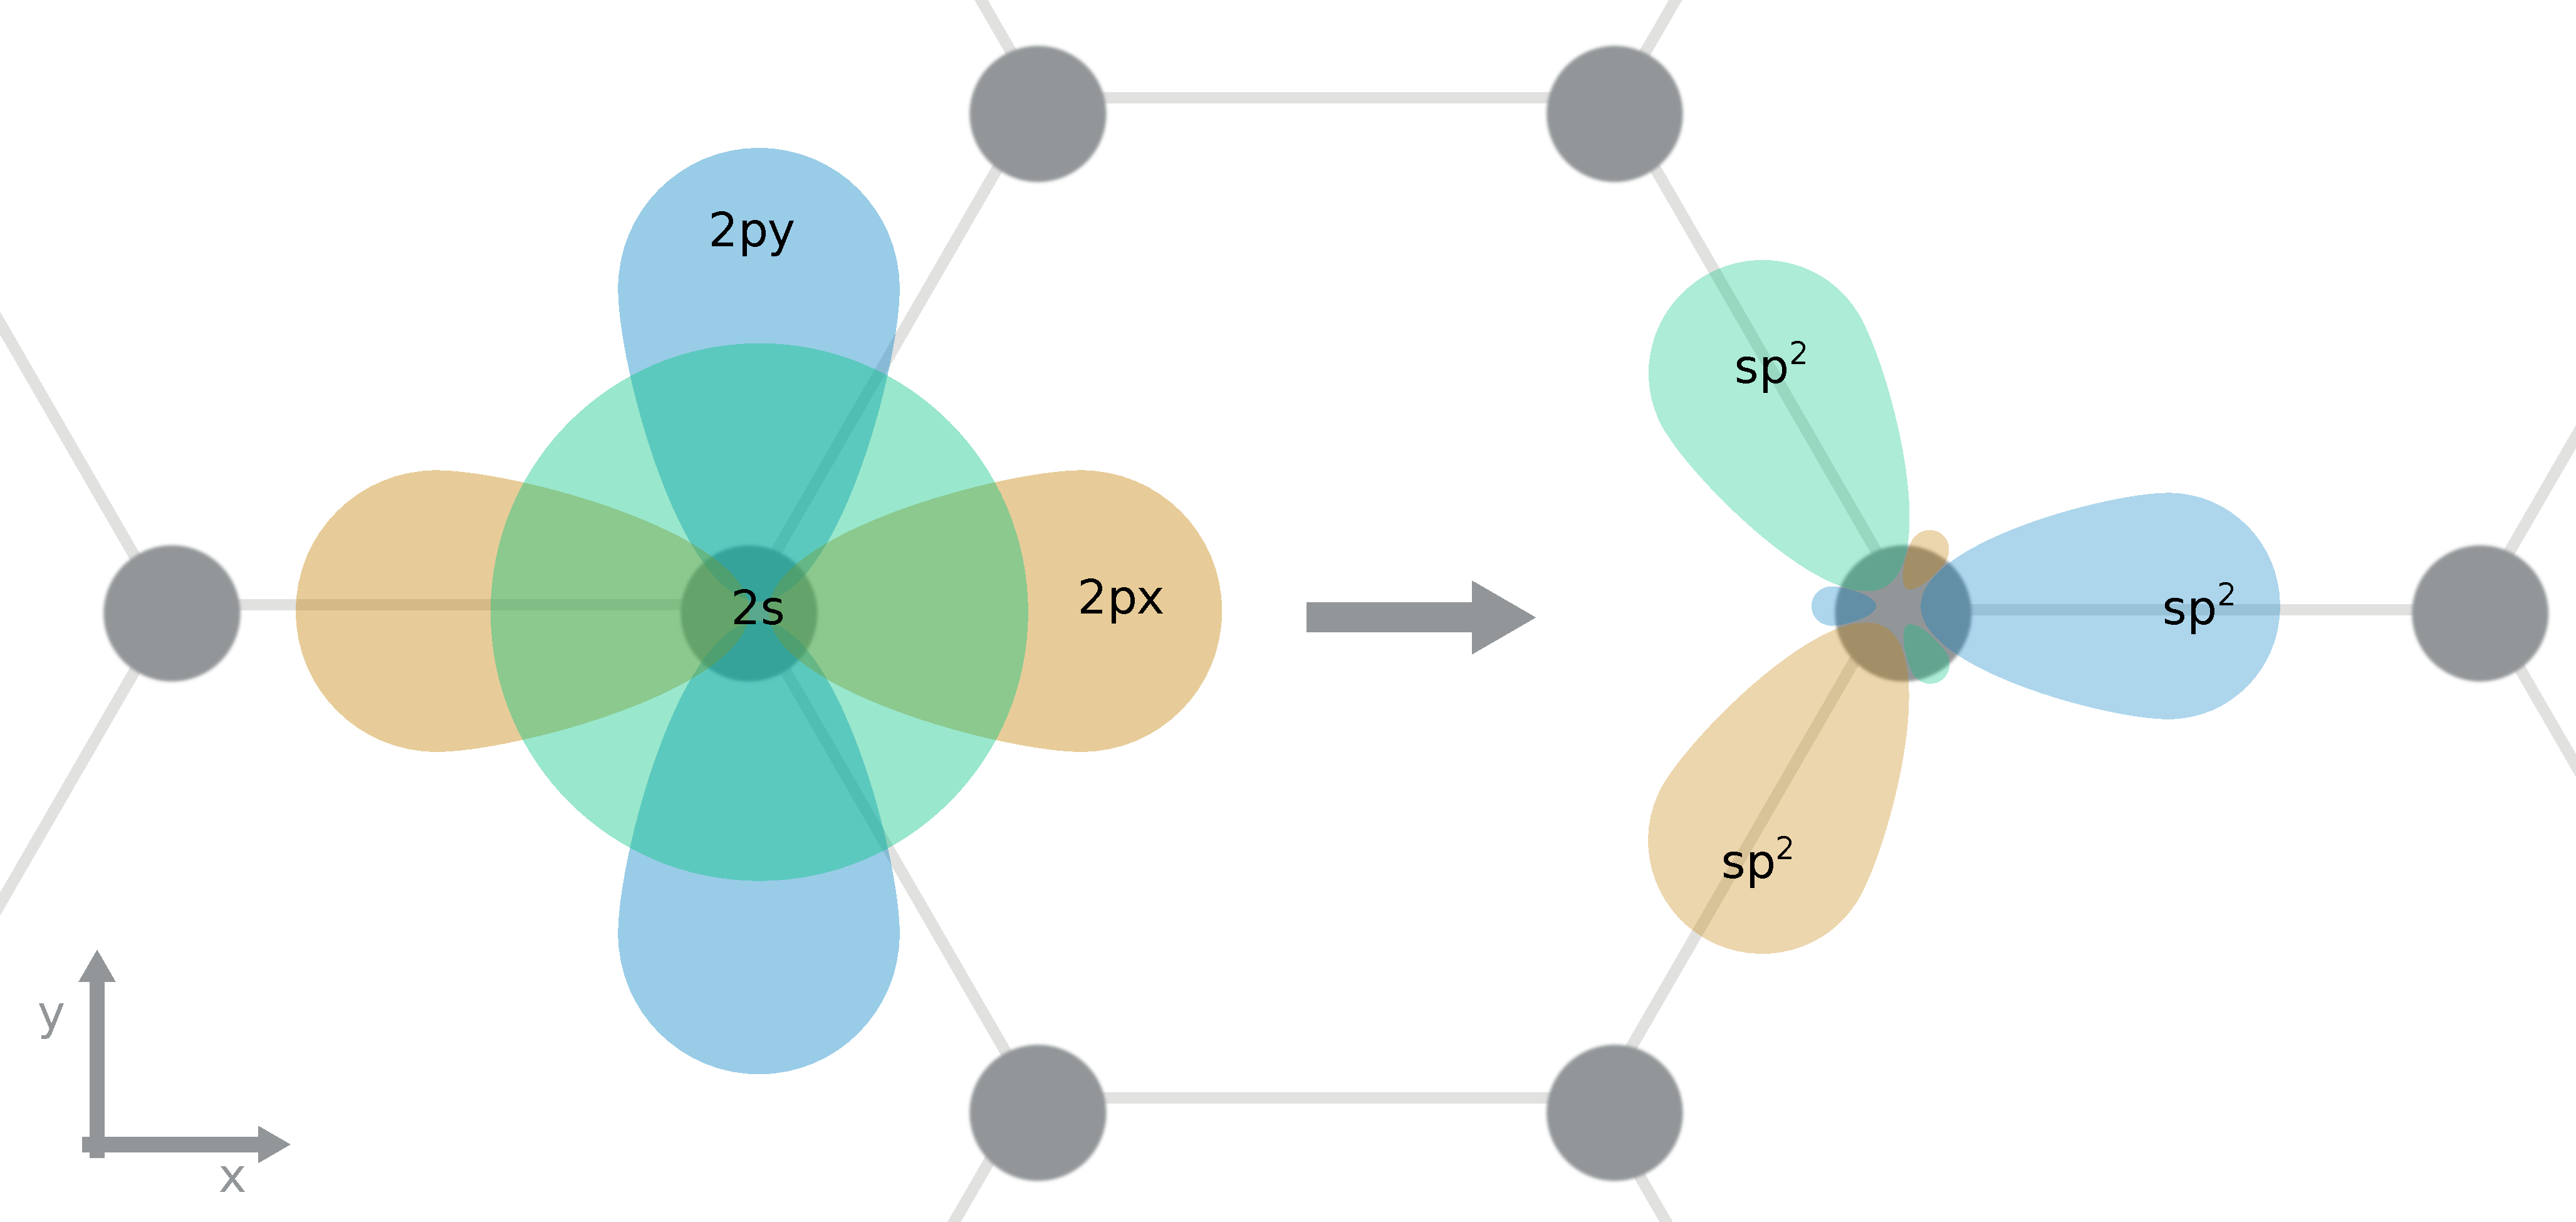
\includegraphics[width=0.75\textwidth]{hybrid.pdf}
	}
	\caption[Hibridización sp2]{Vista frontal. Hibridización sp2 de los átomos de carbono del grafeno. Dos orbitales 2p, junto con el orbital 2s forman tres orbitales sp2 que se disponen de forma planar con un ángulo de 120° entre ellos. Estos orbitales forman enlaces $\sigma$ entre átomos de carbono.}
	\label{fig:sp2_hybrid}
\end{figure}

\begin{figure}[h!]
	\centering
	\fbox{
		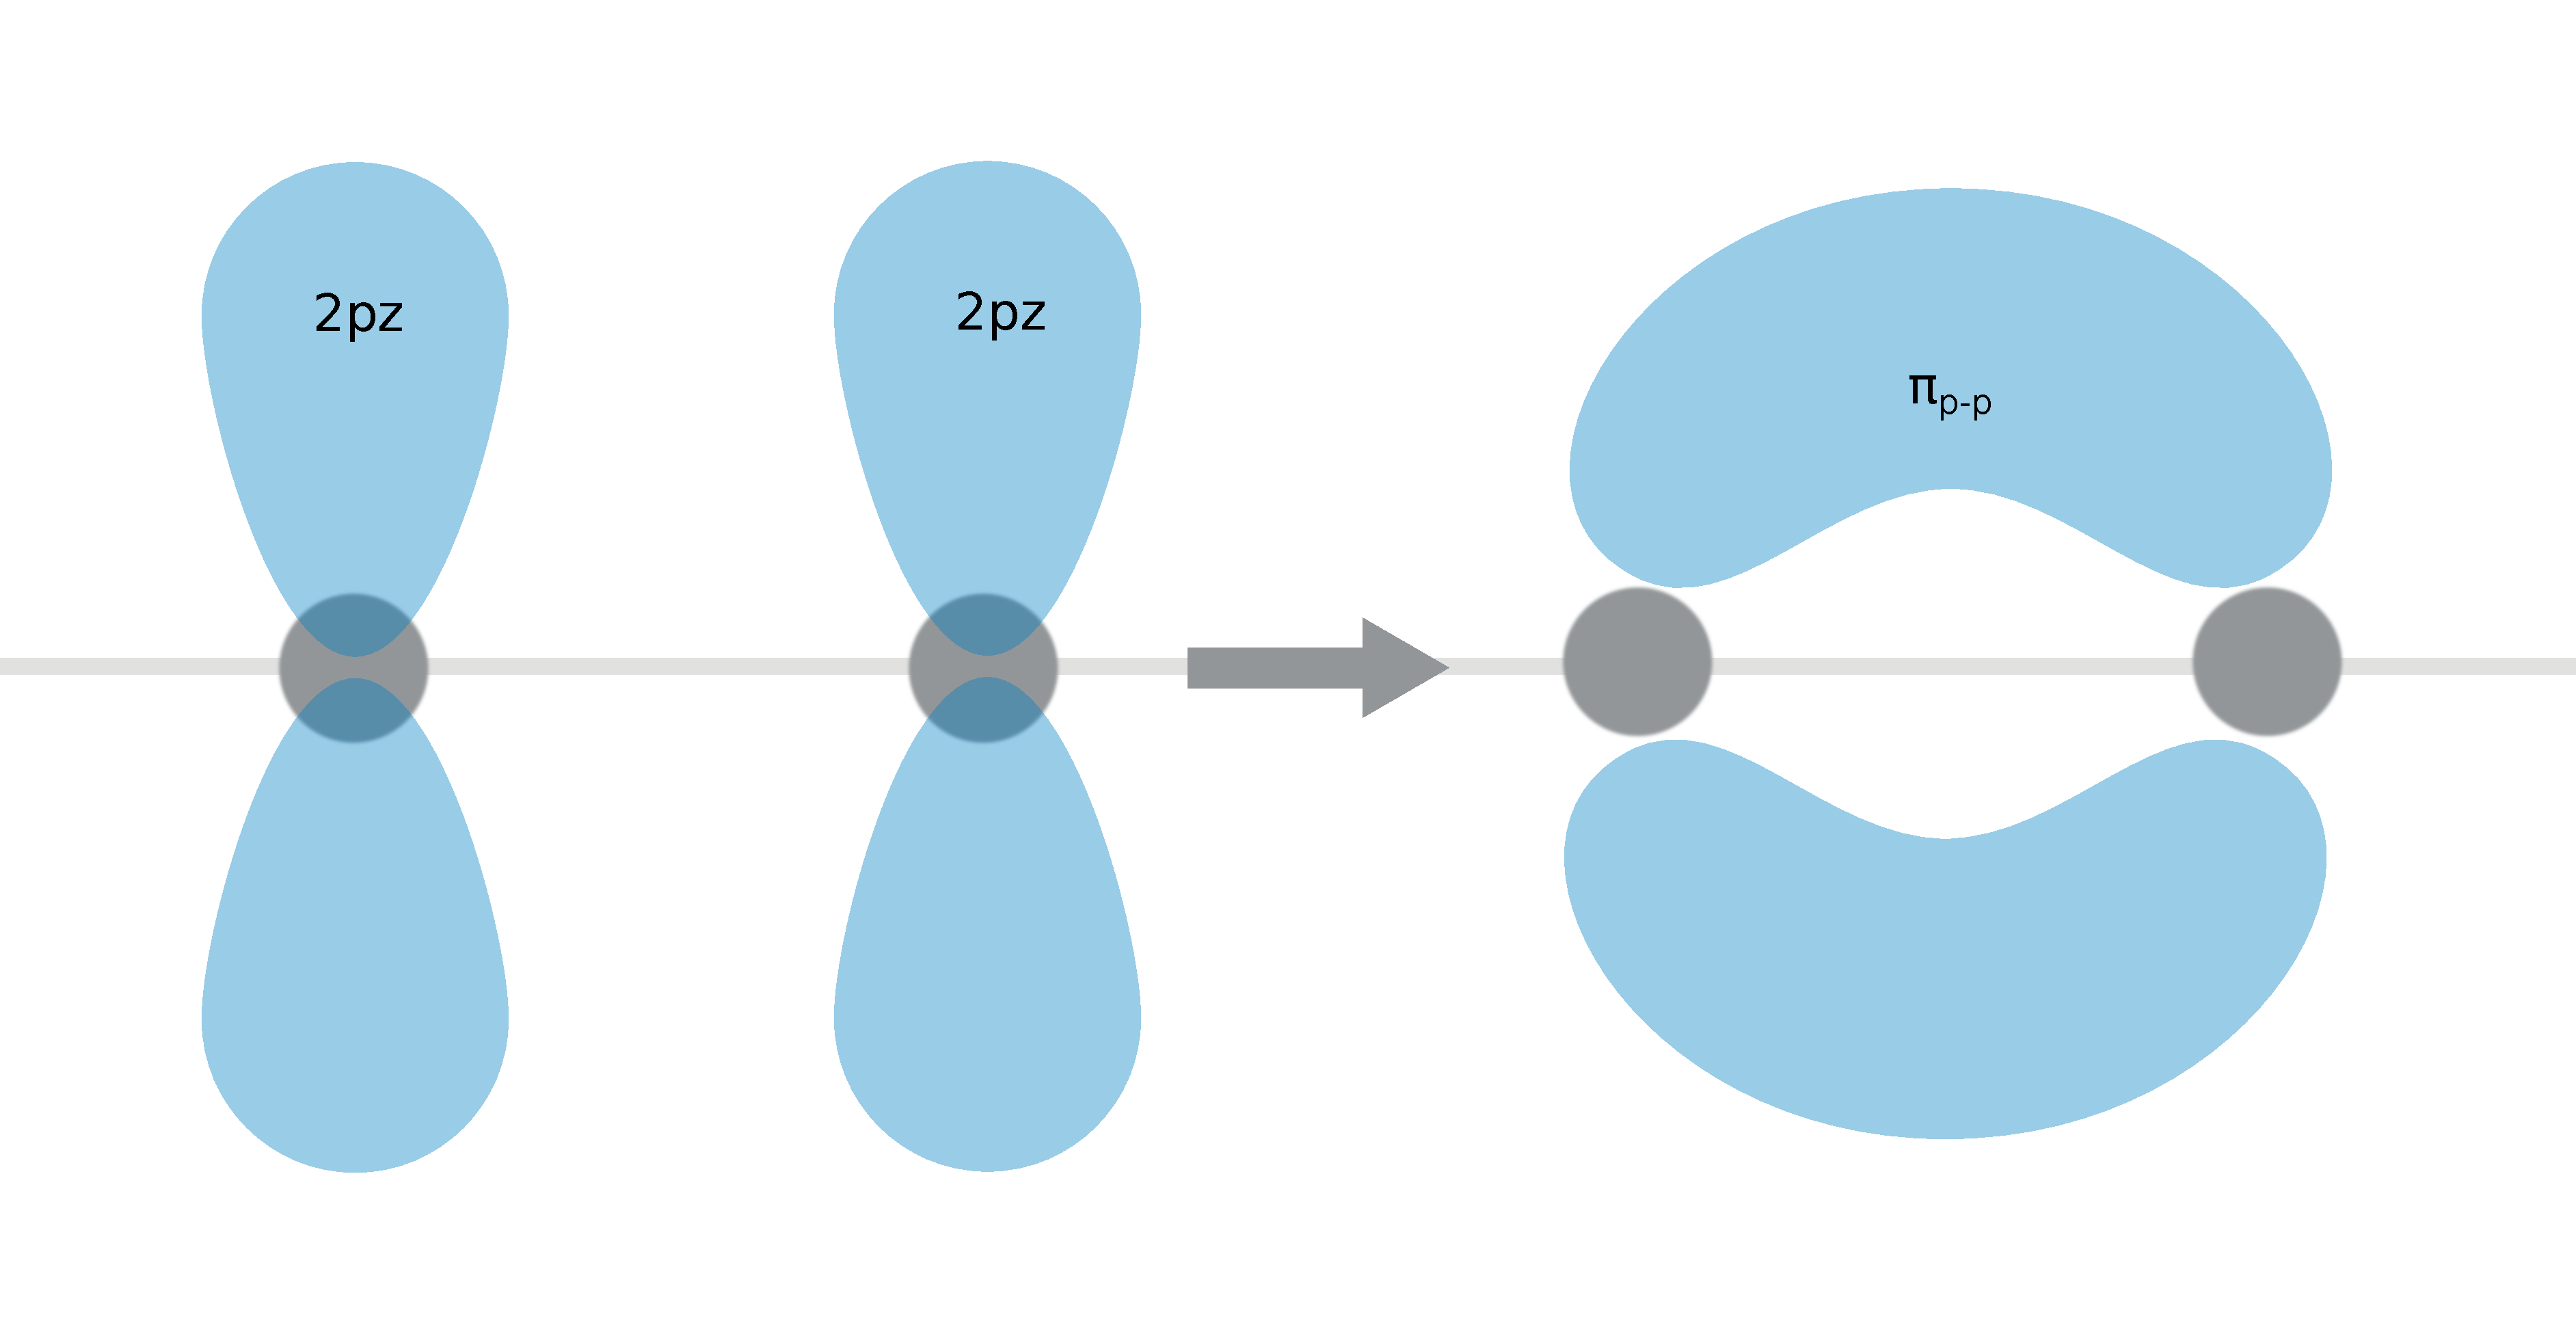
\includegraphics[width=0.75\textwidth]{piorbitals.pdf}
	}
	\caption[Formación de un orbital $\pi$]{Vista lateral de grafeno. Formación de un orbital $\pi_{p-p}$ entre dos átomos de carbono. Junto con el orbital $\sigma$ forman un elace doble entre átomos de carbono.}
	\label{fig:pi_orbitals}
\end{figure}

\clearpage
\section{Caracterización electroquímica}
\label{sec:caracterizacion_electroquimica}
\SCGraphsNoMass{CV_Steel_Disk_No_Material_1}{CV_Steel_Disk_No_Material_2}{0}{16}{1954.91833300000}{Disco de acero sin material}{200}
\SCGraphs{CV_CRGO300517_9}{CV_CRGO300517_10}{0.0004}{10}{3101.89233300000}{Polvo en disco de acero. Masa = 0.4 mg}{0.0002}
\SCGraphs{CV_CRGO300517_3}{CV_CRGO300517_4}{0.0028}{20}{2105.33533300000}{Polvo + PMMA en disco de acero. Masa = 2.8 mg}{0.0002}
\SCGraphs{CV_CRGO300517_11}{CV_CRGO300517_12}{0.0006}{250}{45656.2866670000}{Papel en disco de acero. Masa = 0.6 mg}{0.0001}
\SCGraphs{CV_CRGO300517_13}{CV_CRGO300517_14}{0.0006}{465}{86333.0367000000}{Material liofilizado en disco de acero. Masa = 0.6 mg}{0.0001}

\SCGraphsNoMass{CV_Nickel_Foam_No_Material_1}{CV_Nickel_Foam_No_Material_2}{0}{12}{2399.28233300000}{Espuma de níquel sin material}{200}
\SCGraphs{CV_CRGO300517_5}{CV_CRGO300517_6}{0.0009}{12}{4328.46733300000}{Polvo en espuma de níquel. Masa = 0.9 mg.}{0.0002}
\SCGraphs{CV_CRGO300517_7}{CV_CRGO300517_8}{0.0008}{5}{771.593133000000}{Polvo + PMMA en espuma de níquel. Masa = 0.8 mg}{0.0002}


